\documentclass[tikz,border=5pt]{standalone}
\usepackage{luatexja}
\usepackage[hiragino-pron]{luatexja-preset}
\usepackage{amsmath,amssymb}
\usetikzlibrary{arrows.meta}

\begin{document}
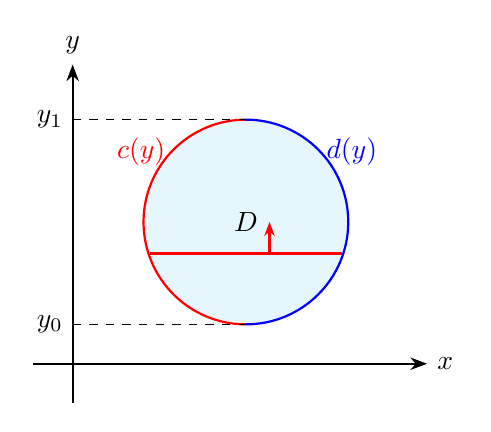
\begin{tikzpicture}

% Parameters
\def\cx{2.2}   % circle center x
\def\cy{1.8}   % circle center y
\def\cr{1.3}   % circle radius

% Axes
\draw[-{Stealth[length=6pt]}, thick] (-0.5,0) -- (4.5,0) node[right] {$x$};
\draw[-{Stealth[length=6pt]}, thick] (0,-0.5) -- (0,3.8) node[above] {$y$};

% Fill region D
\fill[cyan, opacity=0.1] (\cx,\cy) circle (\cr);

% Circle: left half red, right half blue
\draw[red, thick] (\cx,\cy) ++(90:\cr) arc[start angle=90, end angle=270, radius=\cr];
\draw[blue, thick] (\cx,\cy) ++(270:\cr) arc[start angle=270, end angle=450, radius=\cr];

% D label
\node at (\cx,\cy) {$D$};

% Horizontal red arrow inside D at y = 1.4 (inner integral direction: c(y) → d(y))
% Circle at y=1.4: x = cx ± sqrt(cr^2 - (1.4-cy)^2) = 2.2 ± 1.237
\def\ay{1.4}
\pgfmathsetmacro{\ady}{\ay-\cy}
\pgfmathsetmacro{\adx}{sqrt(\cr*\cr - \ady*\ady)}
\draw[red, thick]
  ({\cx-\adx+0.02},\ay) -- ({\cx+\adx-0.02},\ay);
% Up-pointing arrow from middle of red line
\draw[-{Stealth[length=5pt]}, red, thick]
  ({\cx+0.3},\ay) -- ++(0,0.4);

% Dashed lines from circle to y-axis (y0, y1)
\draw[dashed, thin] (0,{\cy-\cr}) -- ({\cx},{\cy-\cr});
\draw[dashed, thin] (0,{\cy+\cr}) -- ({\cx},{\cy+\cr});


% Labels
\node[left] at (0,{\cy-\cr}) {$y_0$};
\node[left] at (0,{\cy+\cr}) {$y_1$};
\node[above left, red] at ({\cx-0.9},{\cy+0.6}) {$c(y)$};
\node[above right, blue] at ({\cx+0.9},{\cy+0.6}) {$d(y)$};

\end{tikzpicture}
\end{document}
